% UQ Gemini Poster - Custom Blue Theme (#093f81 + #d1e2f3)
% Based on: https://github.com/alfurka/gemini-uq

\documentclass[final]{beamer}

% ====================
% Packages
% ====================
\usepackage[T1]{fontenc}
\usepackage{lmodern}
\usepackage[size=custom,width=100,height=75,scale=1.0]{beamerposter}
\usepackage{graphicx}
\usepackage{booktabs}
\usepackage{tikz}
\usepackage{pgfplots}
\pgfplotsset{compat=1.17}
\usepackage[table]{xcolor}  % for \rowcolors

% ====================
% Custom Blue Color Theme (replaces UChicago maroon)
% ====================
\definecolor{primaryblue}{HTML}{093f81}     % Deep blue - main accent
\definecolor{lightblue}{HTML}{d1e2f3}       % Very light blue-gray - backgrounds

\setbeamercolor{palette primary}{fg=black,bg=white}
\setbeamercolor{palette secondary}{fg=black,bg=white}
\setbeamercolor{palette tertiary}{bg=black,fg=white}
\setbeamercolor{palette quaternary}{fg=black,bg=white}
\setbeamercolor{structure}{fg=primaryblue}

% Headline (dark blue bar)
\setbeamercolor{headline}{fg=white,bg=primaryblue}
\setbeamercolor{headline rule}{bg=primaryblue!70!black}

% Blocks
\setbeamercolor{block title}{fg=primaryblue,bg=white}
\setbeamercolor{block separator}{bg=primaryblue}
\setbeamercolor{block body}{fg=black,bg=white}

% Alert blocks (light blue background)
\setbeamercolor{block alerted title}{fg=primaryblue,bg=lightblue}
\setbeamercolor{block alerted separator}{bg=primaryblue}
\setbeamercolor{block alerted body}{fg=black,bg=lightblue!80}

% Items & headings
\setbeamercolor{item}{fg=primaryblue}
\setbeamercolor{heading}{fg=primaryblue}

% Bibliography
\setbeamercolor{bibliography item}{fg=primaryblue}
\setbeamercolor{bibliography entry author}{fg=black}
\setbeamercolor{bibliography entry title}{fg=black}

% ====================
% Load Gemini Theme (after color overrides)
% ====================
\usetheme{gemini}



% ====================
% Layout
% ====================
\newlength{\sepwidth}
\newlength{\colwidth}
\setlength{\sepwidth}{0.025\paperwidth}
\setlength{\colwidth}{0.3\paperwidth}
\newcommand{\separatorcolumn}{\begin{column}{\sepwidth}\end{column}}

% ====================
% Your Content
% ====================
\title{The Impact of Prompt Engineering on Code Generation Accuracy and Hallucination Patterns in Language Models}

\author{Kadin Matotek \texorpdfstring{\\[0.3em] \normalsize Advisor: Dr. Linh B. Ngo}{, Advisor: Dr. Linh B. Ngo}}

\institute[shortinst]{West Chester University, Department of Computer Science}

\footercontent{
  Research conducted at WCU-AIR Lab \hfill
  CSM Dean's Office Student Research Poster Session 2025 \hfill
  \href{mailto:km998744@wcupa.edu}{km998744@wcupa.edu}
}

% Optional logos (adjust paths as needed)
\logoleft{\includegraphics[height=7cm]{figures/wculogo.png}}
\logoright{%
  \begin{minipage}{14cm}
    \centering
    \includegraphics[height=7cm]{figures/icon.png}\\[2em]
    {\Large\color{white}{WCU-AIR Lab}}
  \end{minipage}%
}

% Custom logo overlay (uncomment if you prefer manual placement)
% \addtobeamertemplate{headline}{}
% {
%     \begin{tikzpicture}[remember picture,overlay]
%       \node[anchor=north west,inner sep=3cm] at ([xshift=0cm,yshift=1cm]current page.north west)
%         {\includegraphics[height=5cm]{figures/icon.png}};
%       \node[anchor=north east,inner sep=3cm] at ([xshift=0cm,yshift=2.5cm]current page.north east)
%         {\includegraphics[height=8cm]{figures/icon.png}};
%     \end{tikzpicture}
% }

\begin{document}

\begin{frame}[t]
\begin{columns}[t]
\separatorcolumn

% ==================== Column 1 ====================
\begin{column}{\colwidth}

\begin{block}{Introduction}
Large Language Models (LLMs) have demonstrated remarkable capabilities in code generation, yet their reliability remains a critical concern. This study investigates how different prompt engineering strategies affect model accuracy and hallucination patterns across coding tasks.

\textbf{Research Questions}
\begin{itemize}
  \item How do concise versus verbose instructions impact code generation accuracy?
  \item What types of errors and hallucinations emerge across different model sizes?
  \item How do reasoning strategies (Chain-of-Thought, Direct, Program-Aided) affect performance?
\end{itemize}
\end{block}

\vspace{-1cm}

\begin{block}{Methodology}
We evaluated 5 Qwen2.5-Coder model variants (0.5B to 14B parameters) on 323 programming problems using a systematic prompt engineering framework.

\textbf{Dataset}
\begin{itemize}
  \item \textbf{Source:} Kattis competitive programming platform
  \item Used for rigorous competitions including ICPC
  \item \textbf{Difficulty Range:} 0-2 (on 0-10 Kattis scale)
  \item Focus on fundamental algorithmic challenges
\end{itemize}

\textbf{Experimental Design}
\begin{itemize}
  \item \textbf{Base Instructions:} Concise vs. Verbose (2 options)
  \item \textbf{Reasoning Strategies:} Chain-of-Thought, Direct, Program-Aided (3 options)
  \item \textbf{Problem Decomposition:} None vs. Basic (2 options)
  \item \textbf{Output Formats:} Code only, Explanation + Code, Code + Explanation (3 options)
  \item \textbf{Prompt Variations:} $2 \times 3 \times 2 \times 3 = 36$ unique configurations
  \item \textbf{Total Solutions Generated:} $323 \text{ problems} \times 36 \text{ prompts} \times 5 \text{ models} = 58,140$ code generations
\end{itemize}

\textbf{Evaluation Metrics}
\begin{itemize}
  \item \textbf{Accuracy:} Solutions passing all test cases
  \item \textbf{Error Taxonomy:} 8 hallucination categories, 18 error types
  \item \textbf{Reproducibility:} Dual independent runs
\end{itemize}

\begin{figure}
\centering
\hspace{-2.0cm}
\fcolorbox{lightblue}{white}{\includegraphics[width=1.05\linewidth]{figures/instructions.png}}
\caption{Comparison of base instruction styles: verbose prompts (top) provide detailed explanations while concise prompts (bottom) use minimal, direct language.}
\end{figure}
\end{block}

\end{column}
\separatorcolumn

% =================  Column 2 
\begin{column}{\colwidth}

\begin{alertblock}{Key Finding: Conciseness Advantage}
Across all 18 prompt configuration comparisons, \textbf{concise instructions outperformed verbose ones in 94.4\%} of cases with an average improvement of +1.35\%.

This effect was most pronounced in smaller models, suggesting that verbose instructions may introduce noise that degrades performance.
\end{alertblock}

\begin{block}{Results: Prompt Strategy Performance}

\textbf{Top 3 Configurations} 

\begin{table}
\centering
\small
\begin{tabular}{l l l l r}
\toprule
\textbf{Base} & \textbf{Reasoning} & \textbf{Decomp} & \textbf{Output}       & \textbf{Acc.} \\
\midrule
\rowcolor{lightblue!20}
Concise & Direct    & None  & Code only     & \textbf{33.10\%} \\
Concise & Direct    & None  & Exp + Code    & 32.79\% \\
Concise & CoT       & None  & Exp + Code    & 32.04\% \\
\bottomrule
\end{tabular}
\end{table}

\textbf{Bottom 3 Configurations}

\begin{table}
\centering
\small
\begin{tabular}{l l l l r}
\toprule
\textbf{Base} & \textbf{Reasoning} & \textbf{Decomp} & \textbf{Output}       & \textbf{Acc.} \\
\midrule
Verbose & CoT       & Basic & Code + Exp    & 28.17\% \\
Verbose & PAL       & Basic & Code + Exp    & 27.80\% \\
\rowcolor{lightblue!20}
Verbose & PAL       & Basic & Exp + Code    & \textbf{26.78\%} \\
\bottomrule
\end{tabular}
\end{table}

\vspace{0.5em}
\textit{Max gap: \textbf{+6.32\%}}

\end{block}

\begin{block}{Reasoning Strategy Comparison}
\begin{figure}
\centering
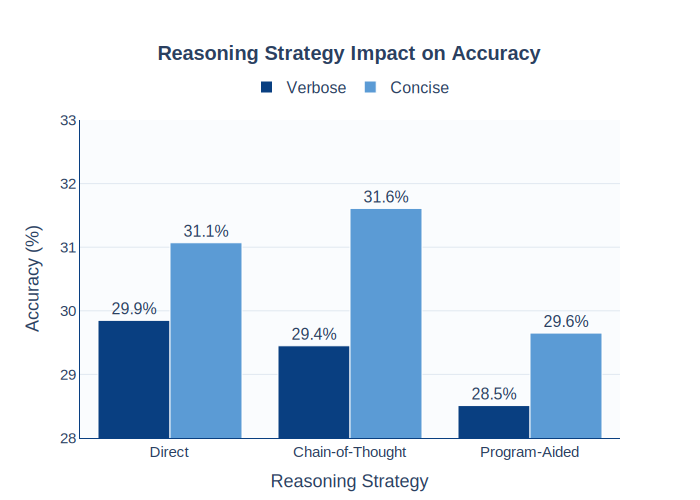
\includegraphics[width=1\linewidth]{figures/reasoning_strategy.pdf}
\caption{Concise prompts consistently outperform verbose across all reasoning strategies (Direct, Chain-of-Thought, and Program-Aided).}
\end{figure}

\end{block}

\end{column}
\separatorcolumn

% ==================== Column 3 ====================
\begin{column}{\colwidth}

\begin{block}{Error and Hallucination Analysis}
We manually defined and annotated 28 distinct error types. Crucially, we observe:

\vspace{0.5em}
\textbf{Highly reproducible hallucination profiles:} Independent runs (v1 vs v2) produce nearly identical error distributions (overlapping solid/dashed lines).

\textbf{Systematic shift with model scale:} Larger models dramatically reduce the dominant error mode while maintaining the same overall failure pattern.
\begin{figure}
\centering
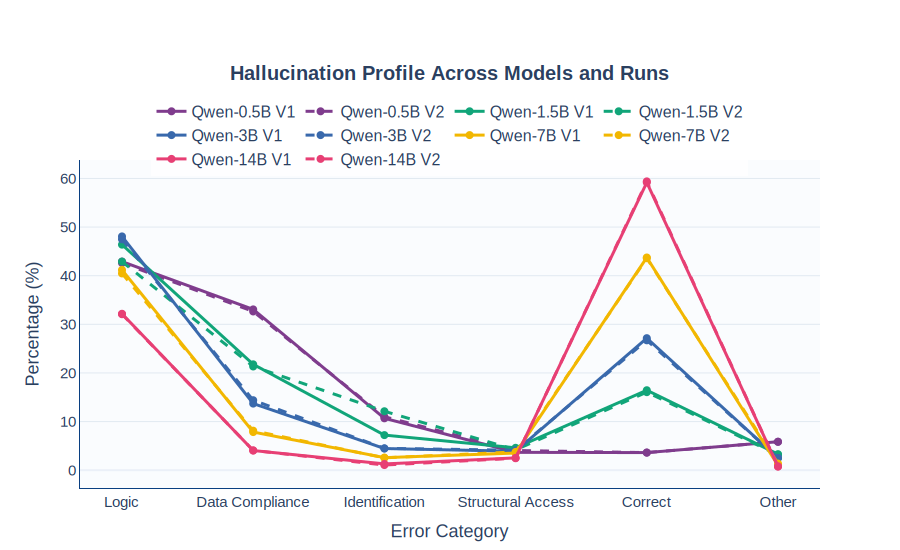
\includegraphics[width=1\linewidth]{figures/hallucination_stability.pdf}
\caption{\textbf{Hallucination profiles are remarkably stable across independent runs} (solid vs dashed lines nearly overlap) but \textbf{shift predictably with model size}.}
\end{figure}

\textbf{Most Common Error Types}
\begin{itemize}
  \item \textbf{Logic Deviation} (41.6\%): Incorrect algorithmic approach
  \item \textbf{ValueError} (12.9\%): Invalid input handling
  \item \textbf{TypeError} (2.9\%): Type mismatches
  \item \textbf{IndexError} (3.1\%): Array boundary violations
  \item \textbf{NameError} (2.8\%): Undefined variables
\end{itemize}

\end{block}

\begin{block}{Conclusions}

\textbf{Key Takeaways}
\begin{itemize}
  \item Concise prompts consistently outperform verbose alternatives
  \item Smaller models are more sensitive to prompt engineering
  \item Logic deviations are the dominant failure mode
  \item Reasoning strategy and output format significantly affect accuracy
\end{itemize}

\textbf{Future Directions}
\begin{itemize}
  \item Extend evaluation to more complex problems (difficulty 3-10)
  \item Test multilingual code generation across Python, Java, C++
  \item Investigate few-shot prompting with example solutions
  \item Develop automated prompt optimization frameworks
\end{itemize}

\end{block}
% \begin{block}{References}
% \nocite{*}
% \small\bibliographystyle{plain}\bibliography{poster}
% \end{block}

\end{column}
\separatorcolumn

\end{columns}
\end{frame}

\end{document}